\documentclass{article}
\usepackage{blindtext}
\usepackage[a4paper, total={6in, 8in}]{geometry}
\usepackage[utf8]{inputenc}
\usepackage{blindtext}
\usepackage{tikz}
\usetikzlibrary{shapes.geometric}
\usepackage[nomessages]{fp}% http://ctan.org/pkg/fp

\begin{document}
\section{Rotation }


\newcommand{\labelStyle}[4]{
\tikzstyle{every node}=[draw,shape=circle,color=red];
%\node (v0) at (0:0) {$v_0$};
\node[top color=white] (v1) at (0:2.5){$#1$} ;
\node[top color=white] (v2) at (90:2.5) {$#2$};
\node[top color=white] (v3) at (2*90:2.5) {$#3$};
\node[top color=white] (v4) at (3*90:2.5) {$#4$};
}

\newcommand{\Square}{
\begin{tikzpicture}
\draw[step=1cm,gray,very thin] (-4,-4) grid (4,4);
\foreach \x in {-4,-3,-2,-1,0,1,2,3,4}
   \draw (\x cm,1pt) -- (\x cm,-1pt) node[anchor=north] {$\x$};
\foreach \y in {-4,-3,-2,-1,0,1,2,3,4}
    \draw (1pt,\y cm) -- (-1pt,\y cm) node[anchor=east] {$\y$};
    \draw [left color=blue,right color=red](0,2) -- (2,0) -- (0,-2) -- (-2,0) -- (0,2);

\labelStyle{V_2}{V_1}{V_4}{V_3};
\end{tikzpicture}
}

\subsection{}{Rotation at angle $0^0$ anticlockwise}

\Square{}\Square{}

\subsection{}{Rotation at angle $90^0$ anticlockwise}

\Square{}
\begin{tikzpicture}
\draw[step=1cm,gray,very thin] (-4,-4) grid (4,4);
\foreach \x in {-4,-3,-2,-1,0,1,2,3,4}
   \draw (\x cm,1pt) -- (\x cm,-1pt) node[anchor=north] {$\x$};
\foreach \y in {-4,-3,-2,-1,0,1,2,3,4}
    \draw (1pt,\y cm) -- (-1pt,\y cm) node[anchor=east] {$\y$};
    \draw [bottom color=blue,top color=red](0,2) -- (2,0) -- (0,-2) -- (-2,0) -- (0,2);
    \labelStyle{V_3}{V_2}{V_1}{V_4};
\end{tikzpicture}

\subsection{Rotation at angle $180^0$ anticlockwise}
\Square{}
\begin{tikzpicture}
\draw[step=1cm,gray,very thin] (-4,-4) grid (4,4);
\foreach \x in {-4,-3,-2,-1,0,1,2,3,4}
   \draw (\x cm,1pt) -- (\x cm,-1pt) node[anchor=north] {$\x$};
\foreach \y in {-4,-3,-2,-1,0,1,2,3,4}
    \draw (1pt,\y cm) -- (-1pt,\y cm) node[anchor=east] {$\y$};
   \draw [right color=blue,left color=red](0,2) -- (2,0) -- (0,-2) -- (-2,0) -- (0,2);
     \labelStyle{V_4}{V_3}{V_2}{V_1};
\end{tikzpicture}

\subsection{Rotation at angle $270^0$ anticlockwise}
\Square{}
\begin{tikzpicture}

\draw[step=1cm,gray,very thin] (-4,-4) grid (4,4);
\foreach \x in {-4,-3,-2,-1,0,1,2,3,4}
   \draw (\x cm,1pt) -- (\x cm,-1pt) node[anchor=north] {$\x$};
\foreach \y in {-4,-3,-2,-1,0,1,2,3,4}
    \draw (1pt,\y cm) -- (-1pt,\y cm) node[anchor=east] {$\y$};
    
\draw [top color=blue,bottom color=red](0,2) -- (2,0) -- (0,-2) -- (-2,0) -- (0,2) ;
\labelStyle{V_1}{V_4}{V_3}{V_2};
\end{tikzpicture}

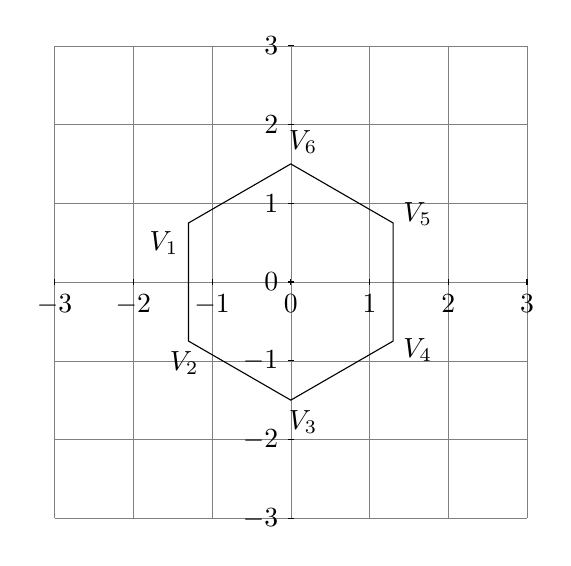
\begin{tikzpicture}
\draw[step=1cm,gray,very thin] (-3,-3) grid (3,3);
\foreach \x in {-3,-2,...,3}
   \draw (\x cm,1pt) -- (\x cm,-1pt) node[anchor=north] {$\x$};
\foreach \y in {-3,-2,...,3}
    \draw (1pt,\y cm) -- (-1pt,\y cm) node[anchor=east] {$\y$};
    
\node (p) [draw,rotate=90,minimum size=3cm,regular polygon, regular polygon sides=6] at (0,0) {};

\foreach \n [count=\nu from 1, remember=\n as \lastn, evaluate={\nu+\lastn}] in {1,2,...,6}
\node[anchor=\n*(360/9)]at(p.corner \n){$V_{\nu}$};
\end{tikzpicture}



\end{document}
